\subsection{Grundlagen des Protokolls}

Für ein Peer-to-Peer Netzwerk gibt es verschiedene Typen. Abbildung \ref{p2p_typen} zeigt
die vier wichtigsten Typen und ihre Unterteilung in unstrukturierte und strukturierte Netzwerke.

\begin{center}
    \captionsetup{type=figure}
    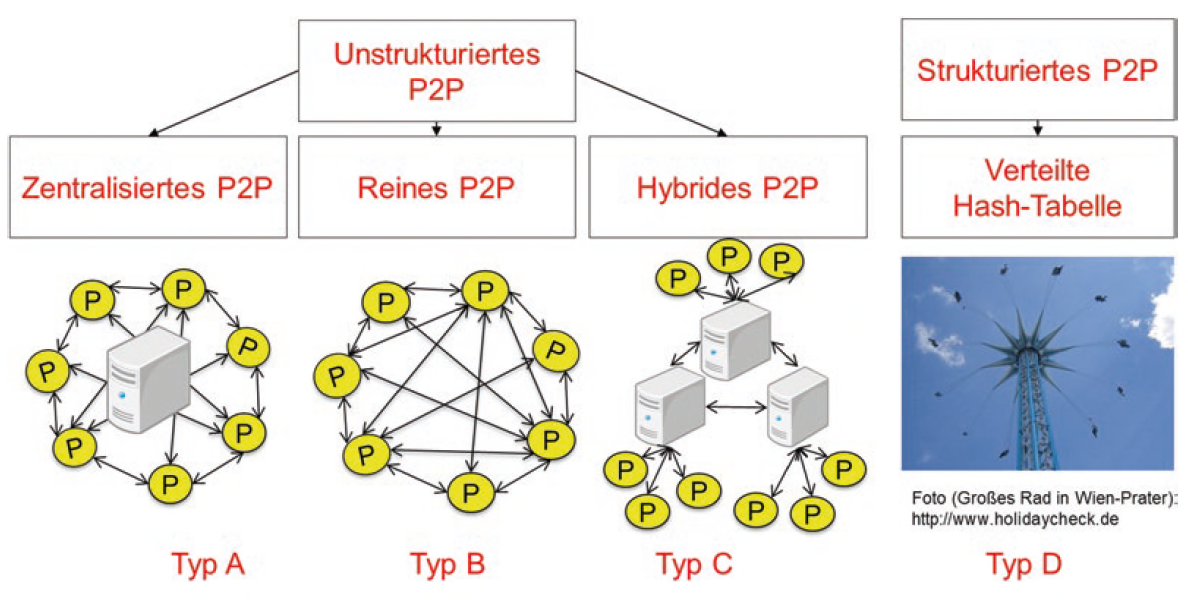
\includegraphics[width=1\linewidth]{images/peer_to_peer_typen.png}
    \captionof{figure}{Typen von Peer-to-Peer Netzwerken \parencite{Luntovskyy_ModRechnernetze}}
    \label{p2p_typen}
\end{center}

\noindent Das Protokoll dieser Arbeit funktioniert auf der Grundlage eines strukturierten 
Peer-to-Peer-Netzwerks.
Grund hierfür ist zum einen, der Fall, dass ein Teilnehmer nicht erreichbar ist, weil er offline ist 
oder weil er sich hinter einem NAT-Gateway befindet. Zum anderen ermöglicht diese Form des Netzwerks
eine effiziente Suche nach Teilnehmern, welche in einem Instant Messaging Protokoll von großer 
Bedeutung ist. Des Weiteren ist ein strukturiertes Peer-to-Peer-Netzwerk skalierbarer als ein
unstrukturiertes Netzwerk, was bedeutet, dass es mit einer großen Anzahl von Teilnehmern umgehen kann.
Die Anordnung der Knoten erfolgt in einem strukturierten Netzwerk nach einem bestimmten Schema.
In dieser Arbeit erfolgt die Anordnung in verteilten Hashtabellen (engl. Distributed Hash Tables).
In dieser Arbeit findet die Topologie der verteilten Hashtabelle Anwendung.
Eine verteilte Hashtabelle
ist eine Datenstruktur, die es ermöglicht, Daten in einem Netzwerk zu speichern und zu suchen.
Die Daten werden in Form von Schlüssel-Wert-Paaren gespeichert. Der Schlüssel ist ein eindeutiger
Bezeichner für den Wert. Der Wert kann ein beliebiger Datensatz sein. Die verteilte Hashtabelle
verteilt die Schlüssel-Wert-Paare auf die Knoten im Netzwerk. Die Zuordnung der Schlüssel-Wert-Paare
zu den Knoten erfolgt über eine Hashfunktion. Die Hashfunktion berechnet aus dem Schlüssel einen
Hashwert. Der Hashwert ist eine Zeichenkette, die aus einer festen Anzahl von Zeichen besteht.
Die Hashfunktion berechnet aus jedem Schlüssel einen Hashwert mit der gleichen Anzahl von Zeichen.
Die Hashwerte werden in einem Zahlenbereich abgebildet.

Um das Problem, welches NAT-Gateways verursachen, zu lösen, wird ein TCP-Relay verwendet. 
Ein TCP-Relay ist ein Server, der als Vermittler zwischen zwei Teilnehmern fungiert, die sich nicht 
direkt verbinden können. Der TCP-Relay ist ein Server, der zwischen den Teilnehmern vermittelt.

